This system comprises an external circle of radius $R$ concentric with an inner ellipse of axes $a,b$, Figure~\ref{fig:II-all}. An explicit parametrization for 3-periodics appears in Appendix~\ref{app:explicit-II}.

\begin{figure}
    \centering
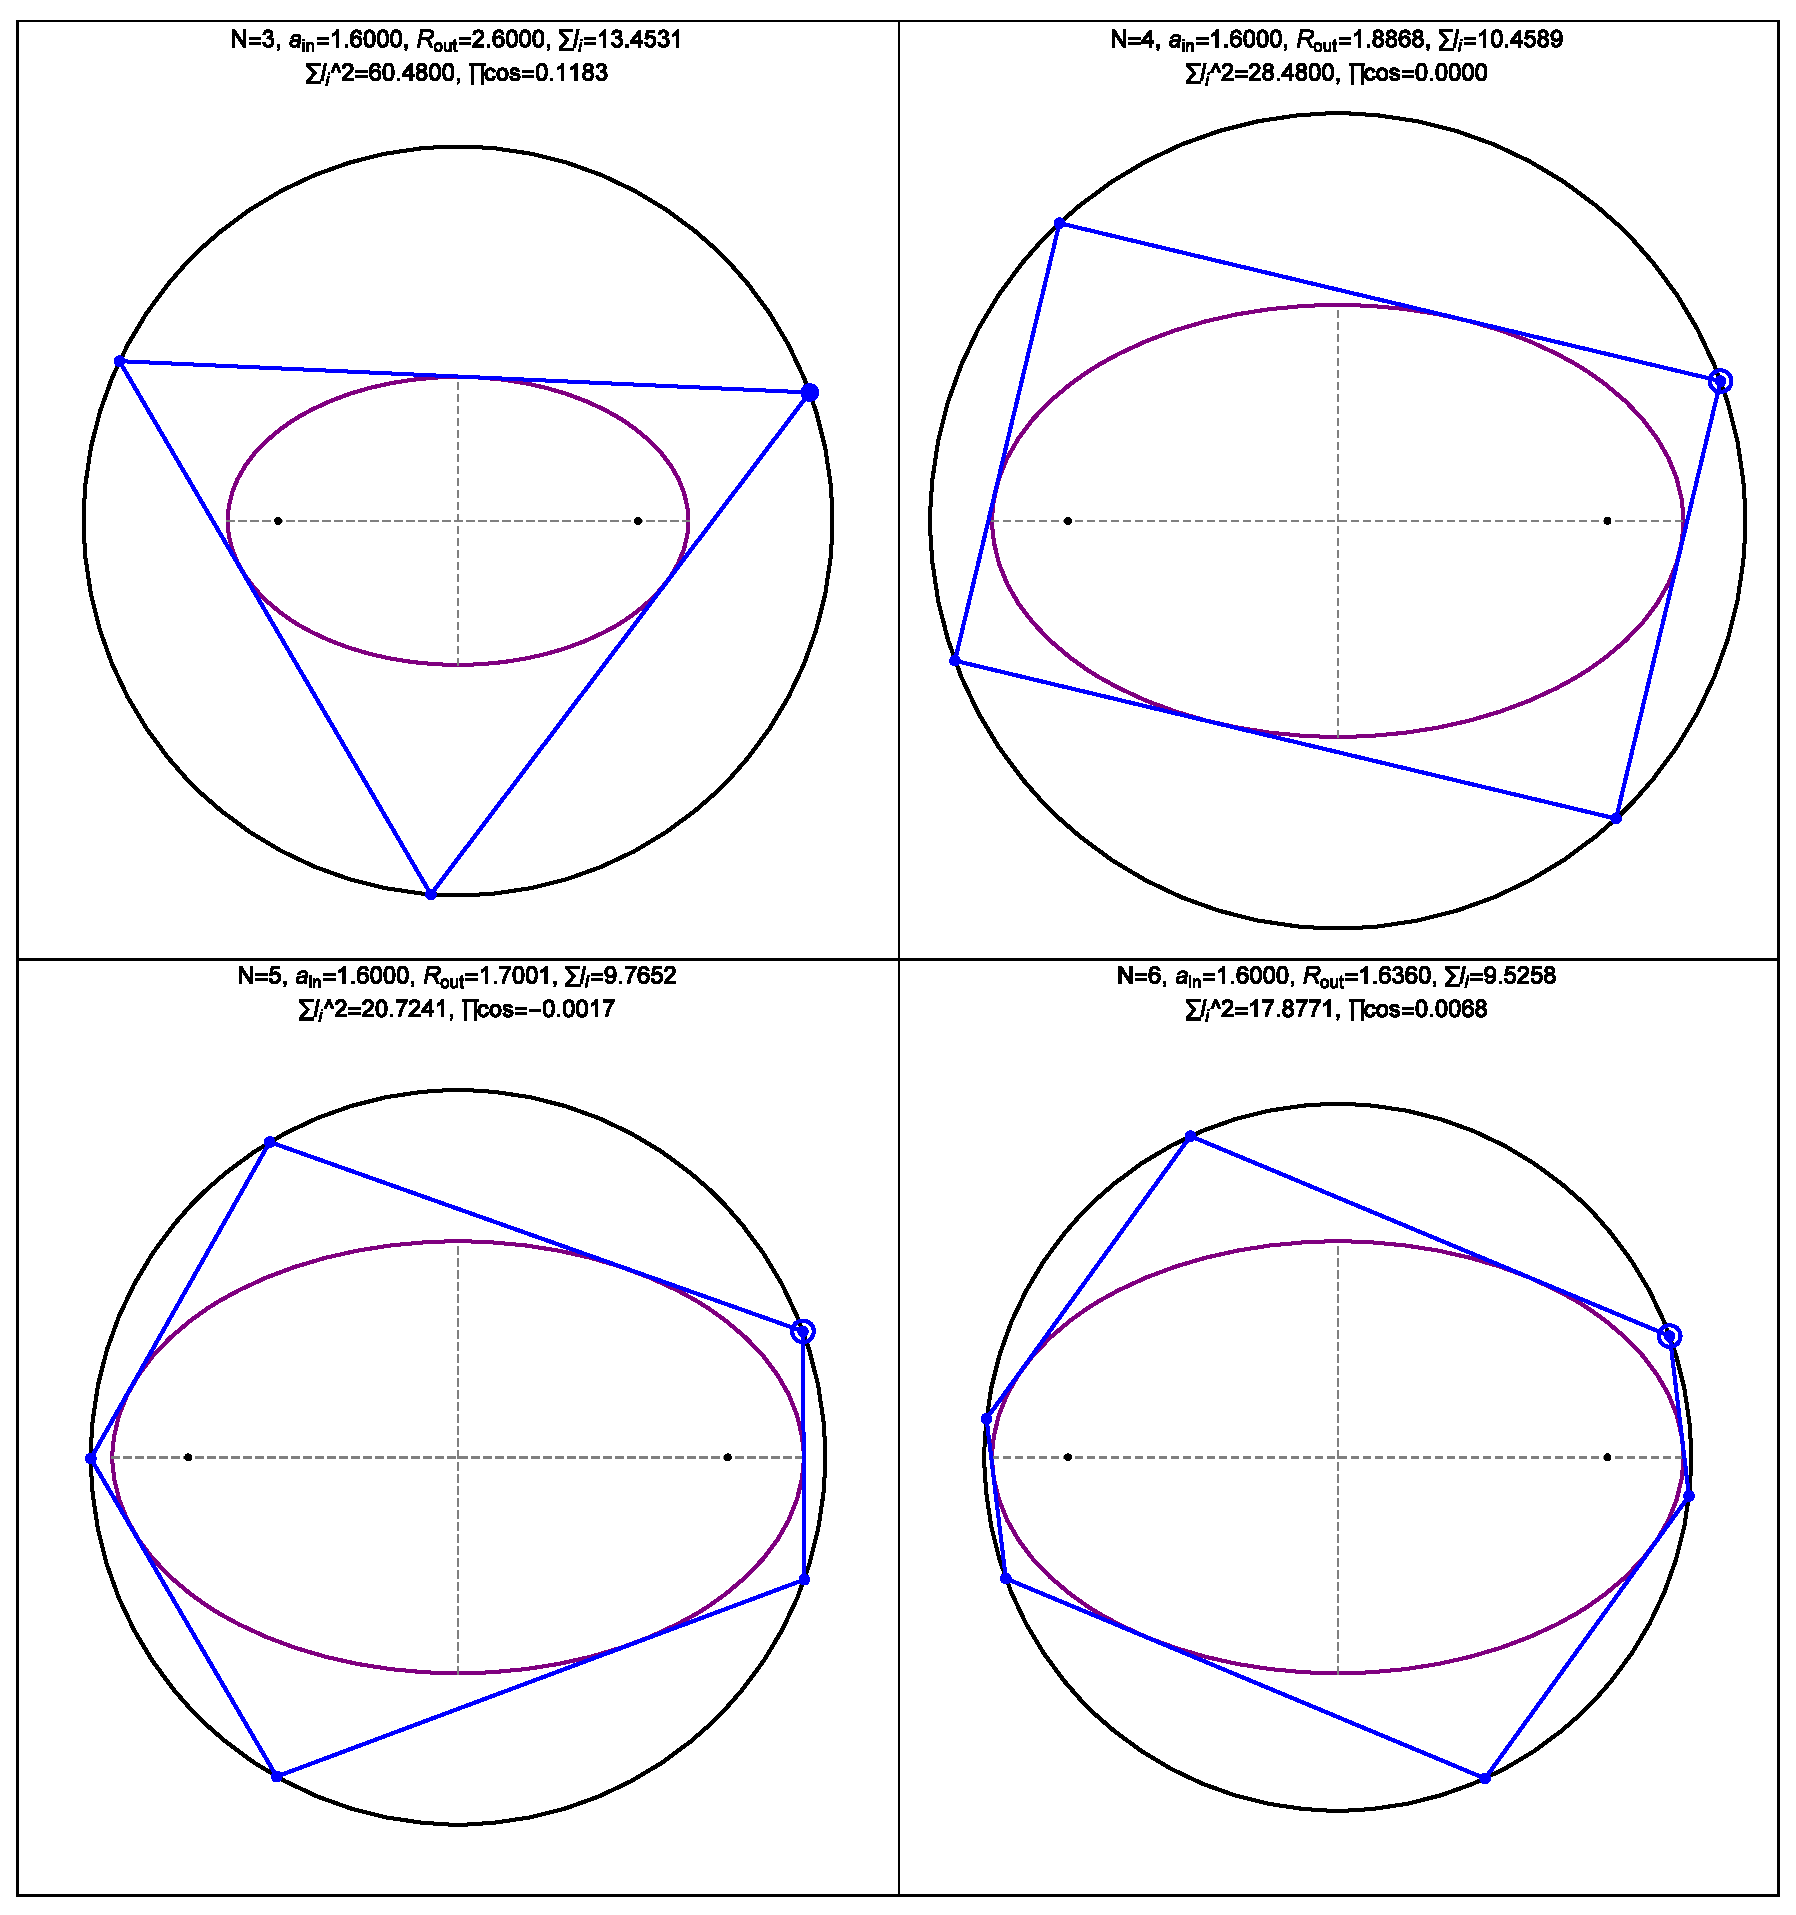
\includegraphics[width=\textwidth]{pics/0020_system_II.eps}
    \caption{System II comprising an external circle and an internal ellipse. Shown are N-periodics for $N=3,4,5,6$.}
    \label{fig:II-all}
\end{figure}

For the $N=3$ case, \eqref{eqn:pair-n3} implies $R=a+b$. By definition $X_3$ is stationary at $O$ and $R$ is the (invariant) circumradius. As shown in Figure~\ref{fig:II-loci}:

\begin{proposition}
The loci of both the orthocenter $X_4$ and nine-point-circle center $X_5$ are concentric circles about $X_3=O$, with radii $d'$ and $2d'$ respectively, where $d'=...$ \textcolor{red}{ronaldo}
\label{prop:II-loci}
\end{proposition}

\begin{proof}

\end{proof}

\begin{figure}
    \centering
    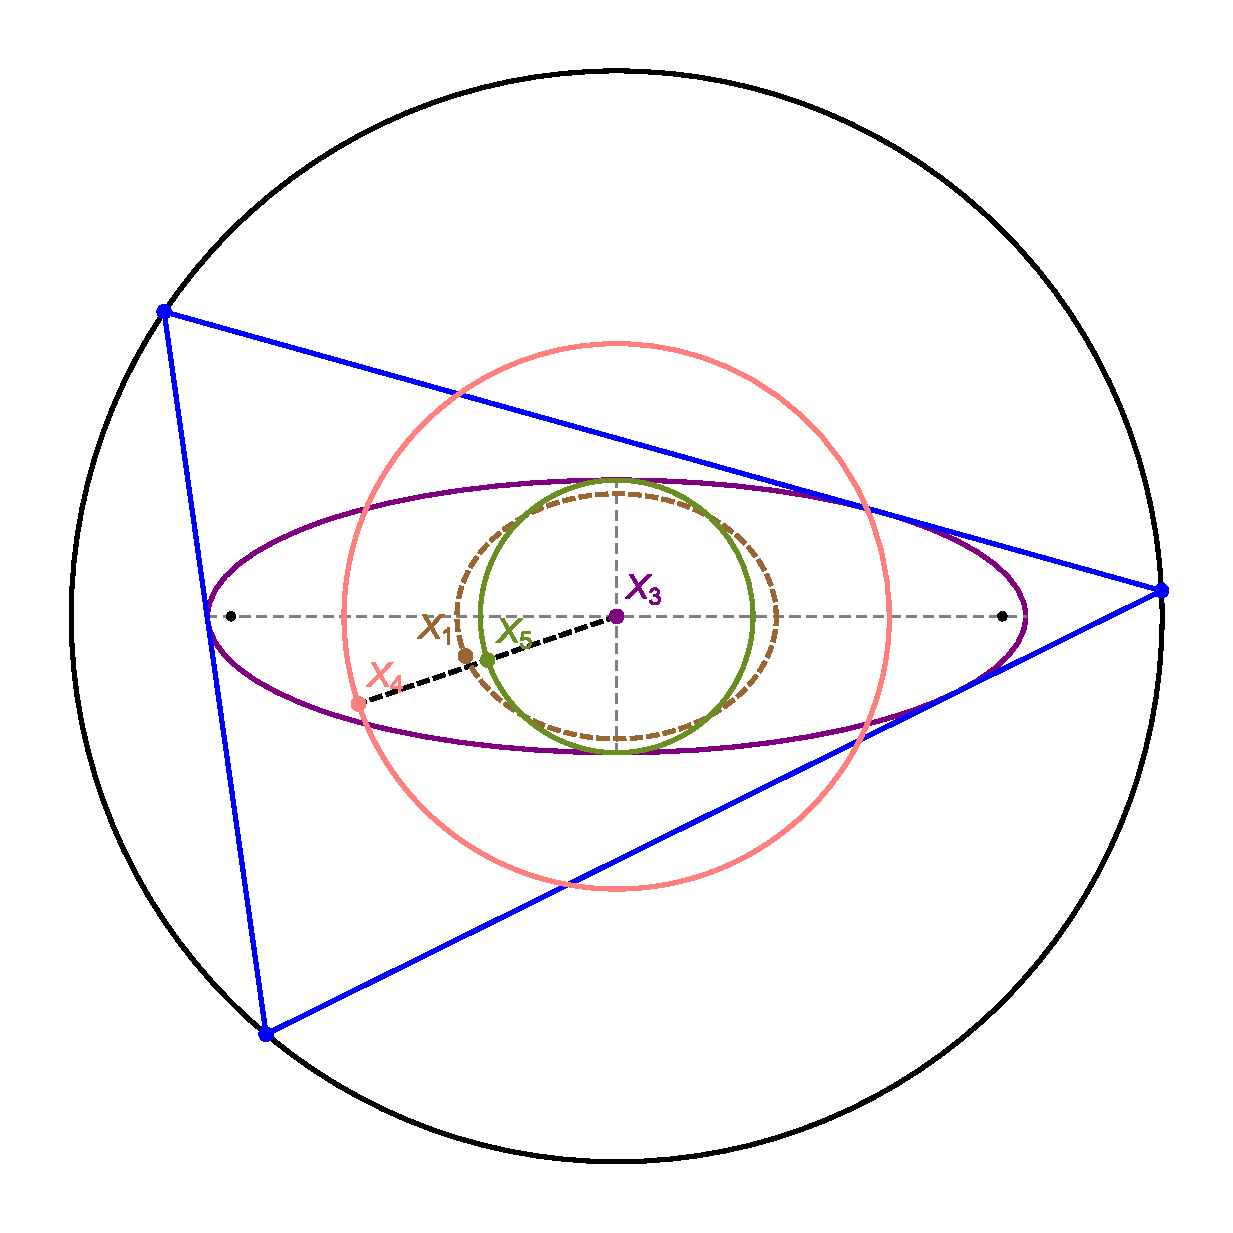
\includegraphics[width=.66\textwidth]{pics/0026_system_II_locus.eps}
    \caption{System II, the $N=3$ case: the loci of both orthocenter $X_4$ (pink) and nine-point center $X_5$ (olive green) are concentric w the external circle (black). Interestingly, the locus of the incenter $X_1$ (dashed brown) is non-elliptic.}
    \label{fig:II-loci}
\end{figure}

However, it can numerically be verified that:

\begin{obs}
The locus of the incenter $X_1$ is non-elliptic. \textcolor{red}{ronaldo, explicit?}
\end{obs}

The orthic triangle has vertices at the feet of perpendiculars dropped from a triangle's orthocenter $X_4$ to the sides \cite{mw}. Referring to Figure~\ref{fig:II-poristic} (left):

\begin{proposition}
Both the inradius and circumradius to the orthic of System II 3-periodics are invariant at $r_h=...$ and $R_h=...$. \textcolor{red}{ronaldo}
\label{prop:II-orthic-radii}
\end{proposition}

\begin{proof}

\end{proof}

\begin{figure}
    \centering
    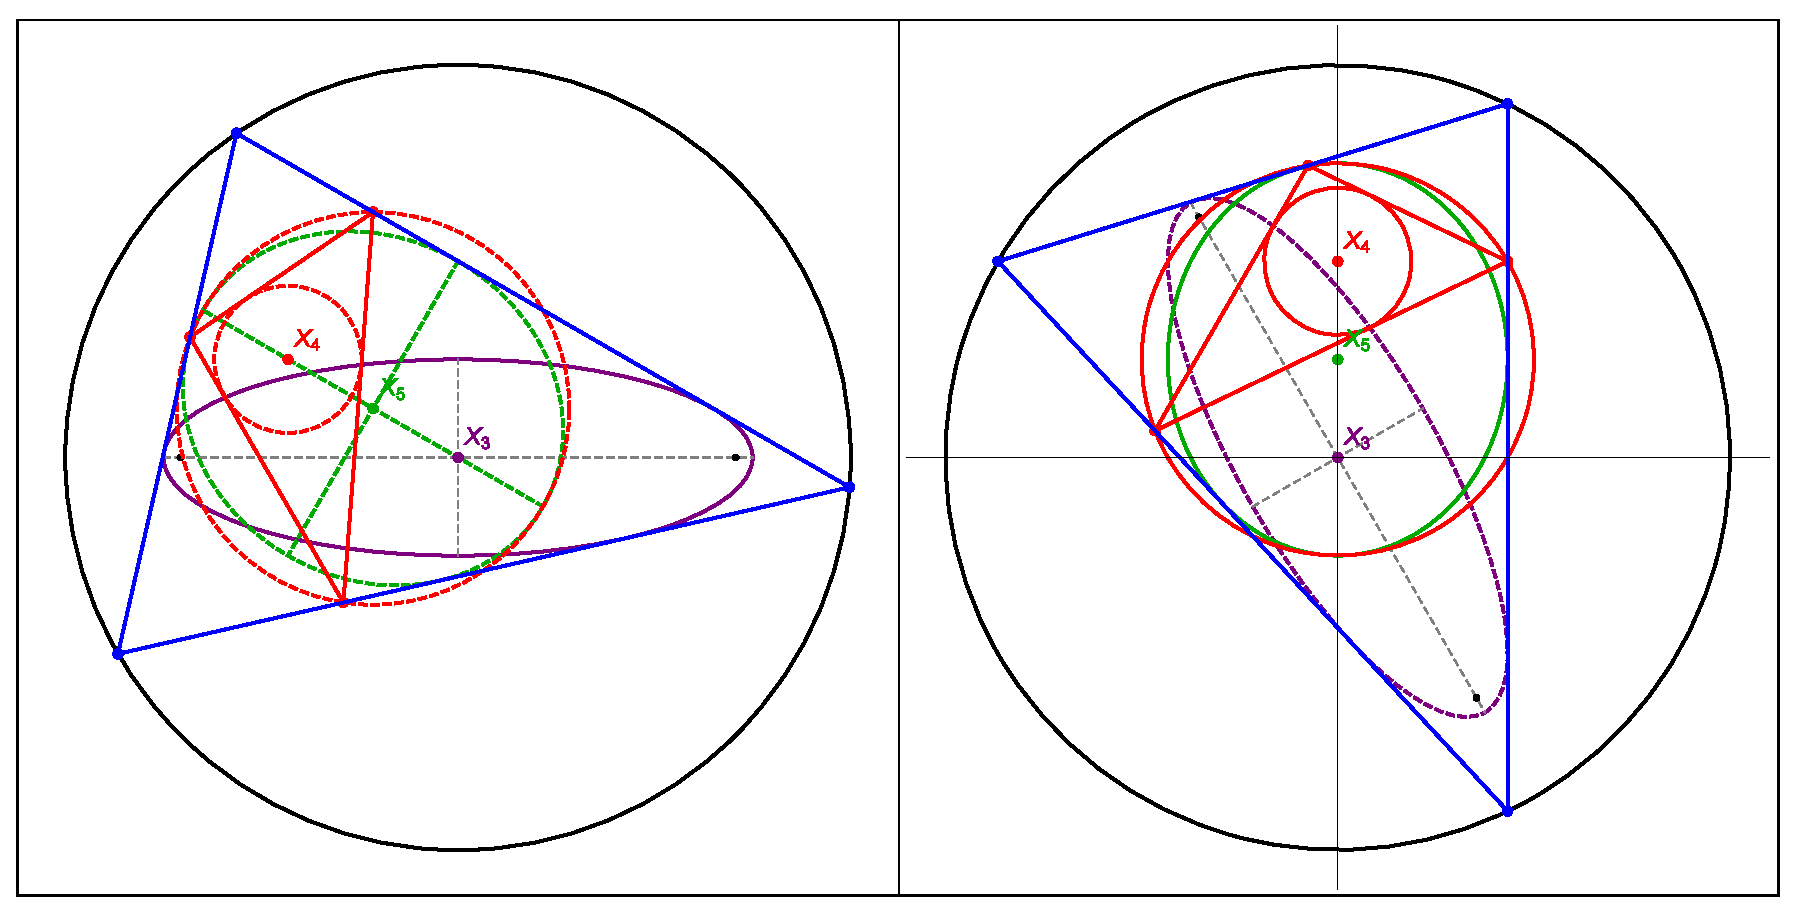
\includegraphics[width=\textwidth]{pics/0025_system_II_poristic.eps}
    \caption{\textbf{Left:} System II 3-periodics (blue), and their orthic triangle (red), whose inradius $r_h$ and circumradius $R_h$ are invariant. The orthic's incircle and circumcircle (both dashed red) are centered on the 3-periodics' orthocenter $X_4$ and nine-point center $X_5$, respectively. Also shown is the rigidly rotating MacBeath inellipse (dashed green) to the 3-periodics, centered on $X_5$ and with foci on $X_3,X_4$. \textbf{Right:} the orthic family is identical (up to rotation), to the Poristic family (red triangle). The original 3-periodics (blue) are the poristics' excentral triangles (blue). Here both incircle and circumcircle (solid red) are stationary. Also stationary is the MacBeath inellipse to the excentrals (green), now its caustic. Consequently, its center $X_5$ and foci $X_3$ and $X_4$ are also stationary. The original outer circle (black on both images) is also stationary on the poristic case, however the original stationary inner ellipse of the Poncelet pair (purple) becomes a rigidly-rotating $X_3$-centered inellipse to the excentrals (dashed purple), whose axes are $R+d$ and $R-d$.}
    \label{fig:II-poristic}
\end{figure}

\begin{lemma}
System II 3-periodics are always acute.
\label{lem:acute}
\end{lemma}

\begin{proof}
\textcolor{red}{ronaldo}
\end{proof}

Let $\mathcal{I}'$ be a (moving) reference frame centered on $X_3$ with one axis oriented toward $X_5$ (or $X_4$ as these 3 are collinear). Referring to Figure~\ref{fig:ellipse-circle-poristic} (right):

\begin{proposition}
With respect to $\mathcal{I}'$, System II 3-periodics are the excentrals to the Poristic family (modulo a rigid rotation about $X_3$).
\end{proposition}

\begin{proof}
$X_5$ is the orthic's $X_3$ \cite{etc}. Since the family is always acute (Lemma~\ref{lem:acute}), $X_4$ is the orthic's $X_1$ \cite{coxeter67}. By  Proposition~\ref{prop:II-loci}, $d'=|X_5-X_3|$ is invariant, i.e., the distance between $X_1$ and $X_3$ of the orthic is invariant. The claim follows from noting $X_3,X_5,X_4$ are collinear \cite{mw} and that the orthic inradius and
circumradius are invariant, Proposition~\ref{prop:II-orthic-radii}. 
\end{proof}

Recall from \cite[Thm 2]{garcia2020-poristic}:

\begin{obs}
The $X_3$-centered inconic to the Poristic excentrals is a rigidly-rotating ellipse with axes $R+d'$ and $R-d'$.
\end{obs}

Which makes sense when one considers the rotating reference frame. Also recall from \cite[Thm 1]{garcia2020-poristic} that:

\begin{obs}
The MacBeath Inconic to the excentrals is stationary with axes $R$ and $\sqrt{R^2-d'^2}$.
\end{obs}

Therefore its focal length is simply $d'=|X_5-X_3|$. Furthermore, because poristic triangles are the image of billiard 3-periodics under a (varying) affine transform \cite[Thm 4]{garcia2020-poristic}, System II 3-periodics will share all scale-free invariants with billiard excentrals, such as product of cosines, ratio of area to its orthic, etc., see \cite{reznik2020-forty}.

Let $s_i$ denote the sidelengths of an $N$-periodic.

\begin{proposition}
The System II $N=3$ family conserves $L_2=\sum{s_i}^2$.
\end{proposition}

\begin{proof}
\textcolor{red}{ronaldo}
\end{proof}

\subsection*{N>3}

Let $K$ as before denote Steiner's {\em Curvature Centroid}. As depicted in Figure~\ref{fig:II-krummungs}:

\begin{conjecture}
$K$ is stationary at $O$ for System II N-periodics, for all N.
\end{conjecture}

Let $A'$ be the area of a system II N-periodic, and $A_k'$ be area of the pedal polygon of the $N$-periodic with respect to $K$, Figure~\ref{fig:II-krummungs}.

\begin{conjecture}
Given any $N$, the ratio $A_k'/A'$ for System II N-periodics is invariant over the family and only depends on $N$.
\end{conjecture}

\begin{figure}
    \centering
    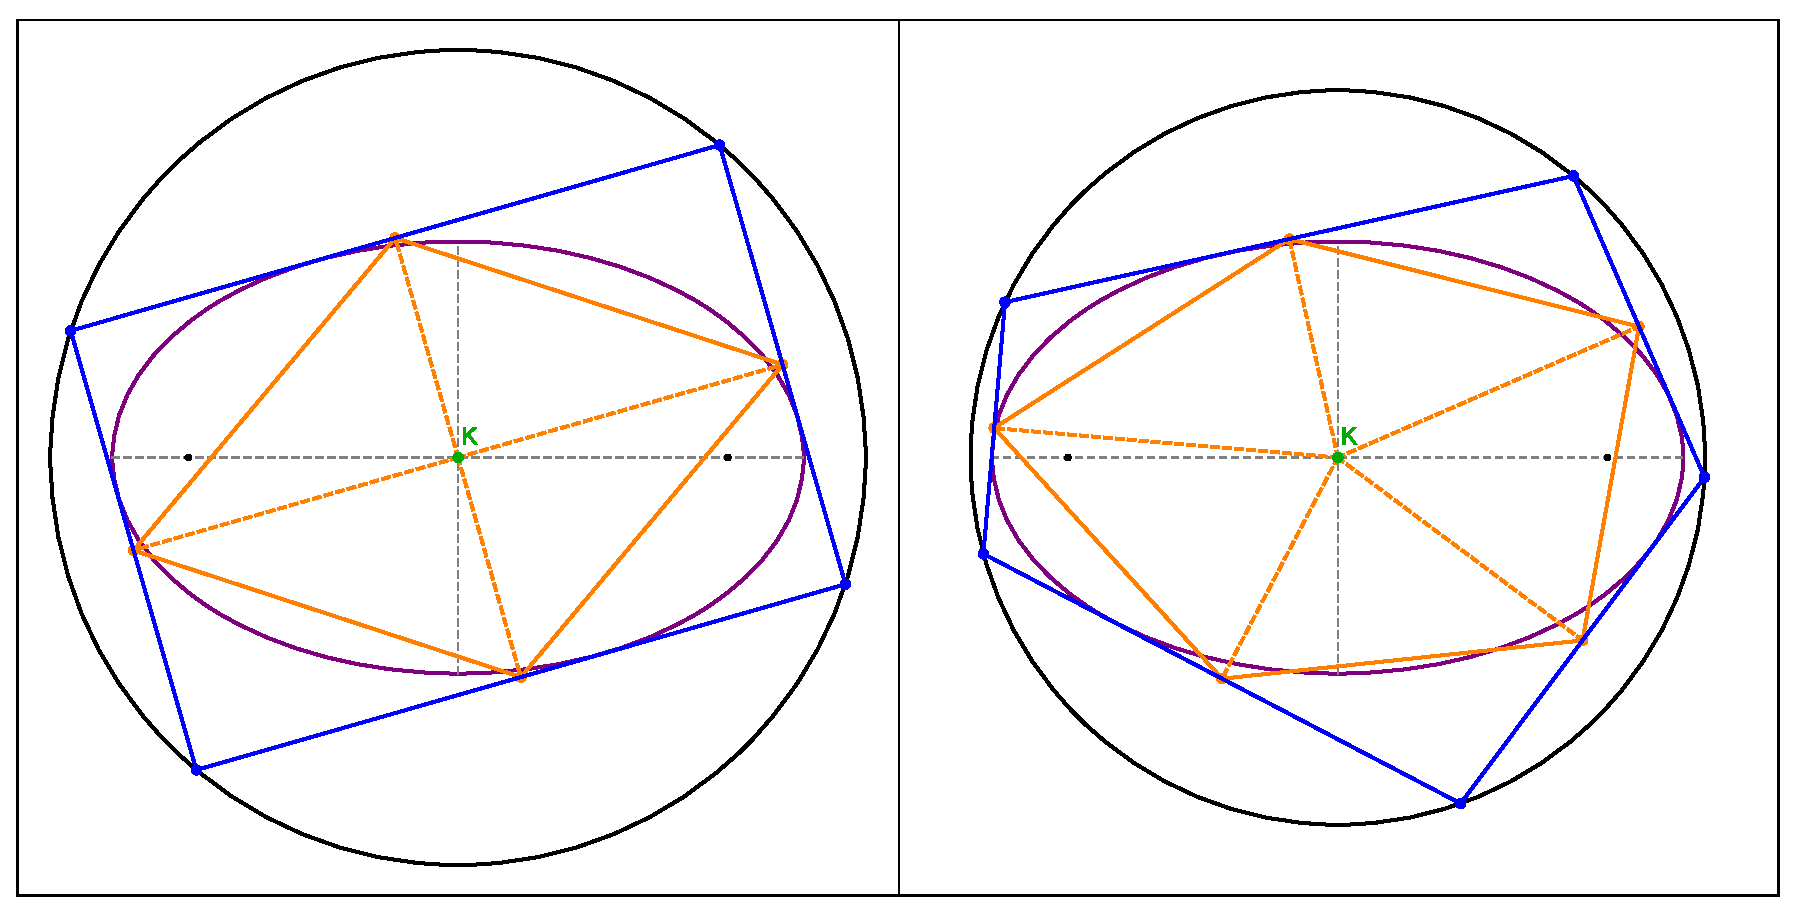
\includegraphics[width=\textwidth]{pics/0027_system_II_pedals.eps}
    \caption{System II, $N=4$ (left) and $N=5$ (right). For any $N$, the Steiner Curvature Centroid $K$ will be stationary at $O$. Also the area ratio of the $K$-pedal (orange) to the $N$-periodic is invariant for all $N$.}
    \label{fig:II-krummungs}
\end{figure}

Referring to  \cite{reznik2020-forty} for a 40+ list of Elliptic Billiard N-periodic invariants, we verify experimentally:

\begin{conjecture}
N-Periodics in System II conserve all scale-free invariants displayed by the excentrals of billiard N-periodics, product of cosines, area ratio (resp. product) to N-periodics for odd (resp. even), etc. Furthermore, these also conserve $L_2=\sum{s_i}^2$.
\end{conjecture}